%\section{ТЗ:}



\begin{lstlisting}[label=some-code,caption=Программа 1.]
#include <stdio.h>
#include <unistd.h>
#include <stdlib.h>

#define OK 0
#define ERROR 1
#define SLEEP_TIME 2
#define ERROR_FORK -1

int main()
{
	int childpid_1, childpid_2;

	// Первый процесс.
	// Создается дочерний процесс
	if ((childpid_1 = fork()) == ERROR_FORK)
	{
		// Если при порождении процесса произошла ошибка.
		perror("Can\'t fork.\n");
		return ERROR;
	}
	else if (!childpid_1)
	{
		// Это процесс потомок.
		sleep(SLEEP_TIME);
		printf("First child: id: %d ppid: %d  pgrp: %d\n", getpid(), getppid(), getpgrp());
		exit(OK);
	}

	// Аналогично 2 процесс.
	if ((childpid_2 = fork()) == ERROR_FORK)
	{
		perror("Can\'t fork.\n");
		return ERROR;
	}
	else if (!childpid_2)
	{
		// Это процесс потомок.
		sleep(SLEEP_TIME);
		printf("Second child: id: %d ppid: %d  pgrp: %d\n", getpid(), getppid(), getpgrp());
		exit(OK);
	}

	printf("Parent: id: %d pgrp: %d child1: %d child2: %d\n", getpid(), getpgrp(), childpid_1, childpid_2);

	return OK;
}
\end{lstlisting}

\begin{figure}[ht!]
	\centering{
		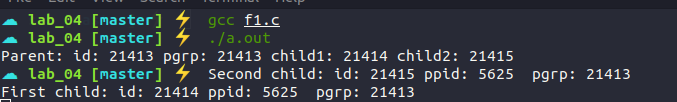
\includegraphics[width=0.8\textwidth]{img/1_1.png}
		\caption{Результат работы программы 1.} }
\end{figure}

\begin{figure}[ht!]
	\centering{
		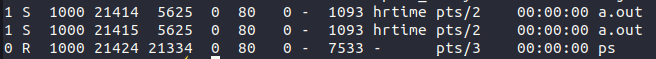
\includegraphics[width=0.8\textwidth]{img/1_2.png}
		\caption{Новый parent pid у процессов-сирот.} }
\end{figure}

\begin{figure}[ht!]
	\centering{
		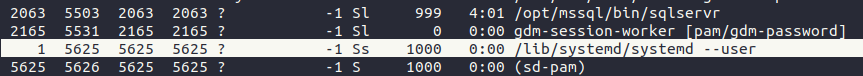
\includegraphics[width=0.8\textwidth]{img/1_3.png}
		\caption{Процесс, который усыновляет процессы-сироты.} }
\end{figure}

\begin{lstlisting}[label=some-code,caption=Программа 2.]
#include <stdio.h>
#include <unistd.h>
#include <sys/wait.h>
#include <stdlib.h>

#define OK 0
#define ERROR 1
#define ERROR_FORK -1
#define SLEEP_TIME 2

void check_status(int status);

int main()
{
	int childpid_1, childpid_2;

	if ((childpid_1 = fork()) == ERROR_FORK)
	{
		// Если при порождении процесса произошла ошибка.
		perror("Can\'t fork.\n");
		return ERROR;
	}
	else if (!childpid_1)
	{
		// Это процесс потомок.
		sleep(SLEEP_TIME);
		printf("First child: id: %d ppid: %d  pgrp: %d\n", getpid(), getppid(), getpgrp());
		exit(OK);
	}

	// Аналогично 2 процесс.
	if ((childpid_2 = fork()) == ERROR_FORK)
	{
		perror("Can\'t fork.\n");
		return ERROR;
	}
	else if (!childpid_2)
	{
		// Это процесс потомок.
		sleep(SLEEP_TIME);
		printf("Second child: id: %d ppid: %d  pgrp: %d\n", getpid(), getppid(), getpgrp());
		exit(OK);
	}

	int status;
	pid_t child_pid;

	child_pid = wait(&status);
	printf("status: %d, child_pid: %d\n", status, child_pid);
	check_status(status);

	child_pid = wait(&status);
	printf("status: %d, child_pid: %d\n", status, child_pid);
	check_status(status);

	printf("Parent: id: %d pgrp: %d child1: %d child2: %d\n", getpid(), getpgrp(), childpid_1, childpid_2);

	return OK;
}

void check_status(int status)
{
	if (WIFEXITED(status))
	{
		printf("Дочерний процесс завершен нормально.\n\n");
		return;
	}

	if (WEXITSTATUS(status))
	{
		printf("Код завершения дочернего процесса %d.\n", WIFEXITED(status));
		return;
	}

	if (WIFSIGNALED(status))
	{
		printf("Дочерний процесс завершается неперехватываемым сигналом.\n");
		printf("Номер сигнала %d.\n", WTERMSIG(status));
		return;
	}

	if (WIFSTOPPED(status))
	{
		printf("Дочерний процесс остановился.\n");
		printf("Номер сигнала %d.", WSTOPSIG(status));
	}
}
\end{lstlisting}


\begin{figure}[ht!]
	\centering{
		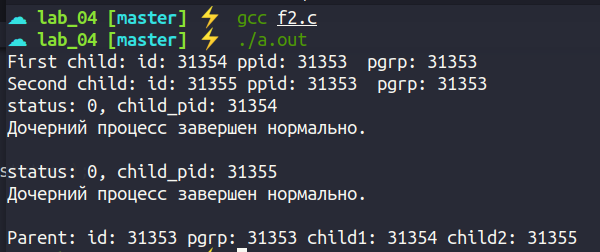
\includegraphics[width=0.8\textwidth]{img/2.png}
		\caption{Результат работы программы 2.} }
\end{figure}


\begin{lstlisting}[label=some-code,caption=Программа 3.]
#include <stdio.h>
#include <sys/wait.h>
#include <unistd.h>
#include <stdlib.h>

#define OK 0
#define ERROR 1
#define ERROR_FORK -1
#define ERROR_EXEC -1

void check_status(int status);

int main()
{
	int childpid_1, childpid_2;
	int status;
	pid_t child_pid;

	if ((childpid_1 = fork()) == ERROR_FORK)
	{
		perror("Can\'t fork.\n");
		return ERROR;
	}
	else if (!childpid_1) // Это процесс потомок (ребенок).
	{
		printf("First child: id: %d ppid: %d  pgrp: %d\n", getpid(), getppid(), getpgrp());

		// p - определяет, что функция будет искать "дочернюю"
		// программу     в    директориях,    определяемых
		// переменной среды DOS PATH. Без суффикса p поиск
		// будет  производиться только в рабочем каталоге.
		if (execlp("cat", "cat", "text1.txt", NULL) == ERROR_EXEC)
		{
			perror("First child can\'t exec");
			exit(ERROR);
		}
		exit(OK);
	}

	// Аналогично 2 процесс.
	if ((childpid_2 = fork()) == ERROR_FORK)
	{
		perror("Can\'t fork.\n");
		return ERROR;
	}
	else if (!childpid_2)
	{
		// Это процесс потомок.
		printf("Second child: id: %d ppid: %d  pgrp: %d\n", getpid(), getppid(), getpgrp());
		if (execlp("echo", "echo", "Hello", "world!\n", NULL) == ERROR_EXEC)
		{
			perror("Second child can\'t exec");
			exit(ERROR);
		}
		exit(OK);
	}

	child_pid = wait(&status);
	printf("status: %d, child_pid: %d\n", status, child_pid);
	check_status(status);

	child_pid = wait(&status);
	printf("status: %d, child_pid: %d\n", status, child_pid);
	check_status(status);

	printf("Parent: id: %d pgrp: %d child1: %d child2: %d\n", getpid(), getpgrp(), childpid_1, childpid_2);

	return OK;
}

void check_status(int status)
{
	if (WIFEXITED(status))
	{
		printf("Дочерний процесс завершен нормально.\n\n");
		return;
	}

	if (WEXITSTATUS(status))
	{
		printf("Код завершения дочернего процесса %d.\n", WIFEXITED(status));
		return;
	}

	if (WIFSIGNALED(status))
	{
		printf("Дочерний процесс завершается неперехватываемым сигналом.\n");
		printf("Номер сигнала %d.\n", WTERMSIG(status));
		return;
	}

	if (WIFSTOPPED(status))
	{
		printf("Дочерний процесс остановился.\n");
		printf("Номер сигнала %d.", WSTOPSIG(status));
	}
}
\end{lstlisting}


\begin{figure}[ht!]
	\centering{
		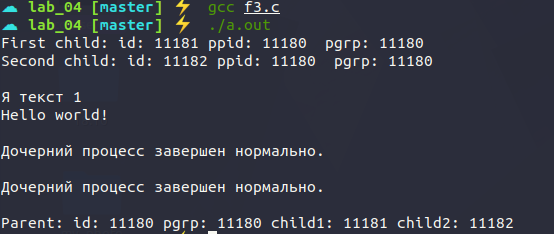
\includegraphics[width=0.8\textwidth]{img/3.png}
		\caption{Результат работы программы 3.} }
\end{figure}

\clearpage

\begin{lstlisting}[label=some-code,caption=Программа 4.]
#include <stdio.h>
#include <stdlib.h>
#include <sys/wait.h>
#include <unistd.h>
#include <string.h>

#define OK 0
#define ERROR 1
#define ERROR_FORK -1
#define ERROR_PIPE -1
#define LEN 32
#define FIRST_TEXT "First child write\n"
#define SECOND_TEXT "Second child write\n"

void check_status(int status);

int main()
{
	int childpid_1, childpid_2;
	int fd[2];

	if (pipe(fd) == ERROR_PIPE)
	{
		perror("Can\'t pipe.\n");
		return ERROR;
	}

	if ((childpid_1 = fork()) == ERROR_FORK)
	{
		// Если при порождении процесса произошла ошибка.
		perror("Can\'t fork.\n");
		return ERROR;
	}
	else if (!childpid_1) // Это процесс потомок.
	{
		close(fd[0]);
		write(fd[1], FIRST_TEXT, strlen(FIRST_TEXT) + 1);
		exit(OK);
	}

	// Аналогично 2 процесс.
	if ((childpid_2 = fork()) == ERROR_FORK)
	{
		perror("Can\'t fork.\n");
		return ERROR;
	}
	else if (!childpid_2) // Это процесс потомок.
	{
		close(fd[0]);
		write(fd[1], SECOND_TEXT, strlen(SECOND_TEXT) + 1);
		exit(OK);
	}

	char text[LEN], text2[LEN];
	pid_t child_pid;
	int status;

	close(fd[1]);

	read(fd[0], text, LEN);
	read(fd[0], text2, LEN);

	printf("Text: %s\n", text);
	printf("Text: %s\n", text2);

	child_pid = wait(&status);
	check_status(status);

	child_pid = wait(&status);
	check_status(status);

	return OK;
}

void check_status(int status)
{
	if (WIFEXITED(status))
	{
		printf("Дочерний процесс завершен нормально.\n\n");
		return;
	}

	if (WEXITSTATUS(status))
	{
		printf("Код завершения дочернего процесса %d.\n", WIFEXITED(status));
		return;
	}

	if (WIFSIGNALED(status))
	{
		printf("Дочерний процесс завершается неперехватываемым сигналом.\n");
		printf("Номер сигнала %d.\n", WTERMSIG(status));
		return;
	}

	if (WIFSTOPPED(status))
	{
		printf("Дочерний процесс остановился.\n");
		printf("Номер сигнала %d.", WSTOPSIG(status));
	}
}
\end{lstlisting}


\begin{figure}[ht!]
	\centering{
		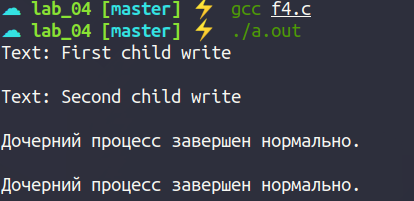
\includegraphics[width=0.8\textwidth]{img/4.png}
		\caption{Результат работы программы 4.} }
\end{figure}

\begin{lstlisting}[label=some-code,caption=Программа 5.]
#include <stdio.h>
#include <stdlib.h>
#include <sys/wait.h>
#include <unistd.h>
#include <signal.h>
#include <stdbool.h> // bool.
#include <string.h>

#define OK 0
#define ERROR 1
#define ERROR_FORK -1
#define ERROR_PIPE -1
#define LEN 32
#define FIRST_TEXT "First child write\n"
#define SECOND_TEXT "Second child write\n"

_Bool flag = false;

void check_status(int status);

void catch_sig(int sig_numb)
{
	flag = true;
	printf("catch_sig: %d\n", sig_numb);
}

int main()
{
	int childpid_1, childpid_2;
	int fd[2];

	signal(SIGINT, catch_sig);
	printf("Parent: нажмите \"CTRL+C\", если хотите получить сообщение.\n\n");
	sleep(2);

	if (pipe(fd) == ERROR_PIPE)
	{
		perror("Can\'t pipe.\n");
		return ERROR;
	}

	if ((childpid_1 = fork()) == ERROR_FORK)
	{
		// Если при порождении процесса произошла ошибка.
		perror("Can\'t fork.\n");
		return ERROR;
	}
	else if (!childpid_1 && flag) // Это процесс потомок.
	{
		close(fd[0]);
		write(fd[1], FIRST_TEXT, strlen(FIRST_TEXT) + 1);
		exit(OK);
	}

	// Аналогично 2 процесс.
	if ((childpid_2 = fork()) == ERROR_FORK)
	{
		perror("Can\'t fork.\n");
		return ERROR;
	}
	else if (!childpid_2 && flag) // Это процесс потомок.
	{
		close(fd[0]);
		write(fd[1], SECOND_TEXT, strlen(SECOND_TEXT) + 1);
		exit(OK);
	}

	if (childpid_1 && childpid_2)
	{
		char text[LEN], text2[LEN];
		pid_t child_pid;
		int status;

		close(fd[1]);

		int a = read(fd[0], text, LEN);

		if (a)
		{
			read(fd[0], text2, LEN);

			printf("Text: %s\n", text);
			printf("Text: %s\n", text2);
		}

		child_pid = wait(&status);
		check_status(status);

		child_pid = wait(&status);
		check_status(status);
	}

	return OK;
}

void check_status(int status)
{
	if (WIFEXITED(status))
	{
		printf("Дочерний процесс завершен нормально.\n\n");
		return;
	}

	if (WEXITSTATUS(status))
	{
		printf("Код завершения дочернего процесса %d.\n", WIFEXITED(status));
		return;
	}

	if (WIFSIGNALED(status))
	{
		printf("Дочерний процесс завершается неперехватываемым сигналом.\n");
		printf("Номер сигнала %d.\n", WTERMSIG(status));
		return;
	}

	if (WIFSTOPPED(status))
	{
		printf("Дочерний процесс остановился.\n");
		printf("Номер сигнала %d.", WSTOPSIG(status));
	}
}
\end{lstlisting}


\begin{figure}[ht!]
	\centering{
		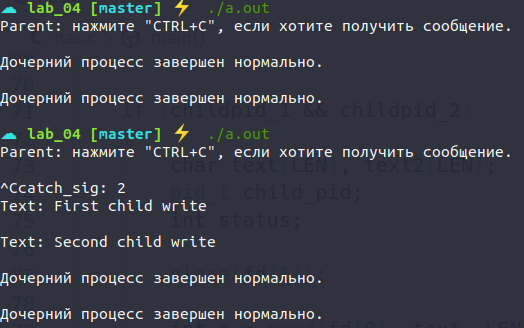
\includegraphics[width=0.8\textwidth]{img/5.png}
		\caption{Результат работы программы 5.} }
\end{figure}
